\documentclass[12pt, letterpaper]{article} 
\usepackage[letterpaper, top=3.71cm, bottom=3.20cm, left=2.86cm, right=2.86cm]{geometry}
%top = 2.44 (header in doc) + 1.27
% bottom 1.42 (footer in doc) + 1.78
\usepackage{graphicx}
\usepackage{array}
\usepackage{placeins}
\PassOptionsToPackage{hyphens}{url}\usepackage{hyperref}
\usepackage{hyperref}
\usepackage{verbatim}
% Square around link (to decide)
\hypersetup{hidelinks}
% Square around link (to decide)
\usepackage{color}
\usepackage{tabularx}
\usepackage{threeparttable}
\usepackage{multirow}
\usepackage{wrapfig}
\usepackage{longtable}
\usepackage{subcaption} % for subfigure environments
\usepackage{booktabs}
\usepackage{nameref}


\title{\vspace{2cm}\textbf{Parallel implementation of Huffman Code using native C++ threads and FastFlow library} \\
        \bigskip
        \Large{
            \medskip
            Parallel and Distributed Systems: Paradigms and Models \\
            \medskip
            University of Pisa \\
            \medskip
            Project Report\\
            \medskip
        }
}
\medskip

\author{
  {Matteo Tolloso}\\
  \texttt{ \scriptsize{m.tolloso@studenti.unipi.it}}\\
  \texttt{\scriptsize{Roll number: 598067}} \\
  %\scriptsize{Artificial Intelligence curriculum}
}

\begin{document}
\nocite{*}
\date{September 1, 2023}
\maketitle

%/////////////////////////////////////
\newpage

\section{Introduction}
The Huffman code is an efficient lossless compression code based on the probability of each character.

To build the optimal code for a specific text we have to:
\begin{enumerate}
    \item count the number of occurences of each character in the text;
    \item build the binary tree that represents the code;
    \item encode the file.
\end{enumerate}

\section{Overview}

We are facing a problem that can be divided in three stages. In particular it is a \textit{data parallel} task, since we have all input available at the beginning of the computation.

\subsection{Counting the number of occurences}
As stated above, the first stage is a counting one. The asymptotic sequential complexity of this part is $\theta(m)$ where $m$ is the number of characters in the file.
From a parallel/distributer point of view this is clearly a \textit{map-reduce} operation.

\paragraph*{Map}
The \textit{Map} part can be execute in parallel dividing the file into chunks, the workers count the occurences in a chunk of the file. 
This operation has to deal with the disk. If we consider the reading of the disk as a sequential operation things became more difficult because it's no longer a data parallel problem but a stream parallel one. In this setting we can describe the process as \texttt{pipe}($reading$, \texttt{farm}($counting$, $nw$)), the completion time of this process is the time needed to read the file from the disk, under the assumption that the farm has the right number of workers to match the speed of the disk. This approach is the one that minimize both the completion time and the number of workers but it causes a lot of comunication overhead, needs some tuning of the chunksize to send and of the scheduler's policy and is in general more complex to implement.

If we instead consider the reading of the disk as a datata parallel operation that consists in moving data from the disk to the main memory, we can use the $Map\ Fusion$ theorem and transform the program in \texttt{map}($read-count$, $nw$). This solution minimize the communication overhead, the completion time and the complexity of the implementation.


Furthermore, the tests that i did mapping the file in main memory and reading it with multiple threads, showed that the parallelization
also improves the performance of the read operation. This is probably due to how the SSD works and the caching syestems. 

\paragraph*{Reduce}
After the \textit{Map} operiation we end up with a number of counts vectors equal to the number of chunks the file was divided into (that in our case is equal to the number of workers). The \textit{Reduce} operation is again a parallel one, this time each reducer takes a subset of the alphabet and sums the occurences of each character in that subset. It's useless to have a number of workers greater than the number of different characters in the file.

\subsection{Building the binary tree}
The second stage is the building of the binary tree. This is a more difficult operation to parallelize since 
most of the operations are sequential. Furthermore, the complexity of this stage is $\theta(A \times log (A))$  where 
$A$ is the number of differtent symbols (128), so basically it is a constant in our case. Tests showed that the time needed for this stage is competely negligible with respect to the other stages.

\subsection{Encoding the file}
The last stage is the \textit{encoding} of the file. This is a \textit{Map} operation, since each character has to be replaced with its code and writed on the disk. We can make a similar reasoning as the one made for the counting stage about the $Map\ Fusion$ theorem.

Unfortunately, the lenght of the final text can only be known after each character has been encoded (because the encoding of each character
has a different lenght), so the actual writing needs a step of syncronization. I solved this problem dividing this stage in thread parts:
\begin{enumerate}
    \item \textit{encoding}: each worker encodes a chunk of the file.
    \item \textit{balancing}: the encoded chunks sizes are made multiple of 8 and the the index where the writing should start is computed. This is a sequential syncronization step but the time needed is negligible.
    \item \textit{compressing and writing}: each worker takes a chunk of the encoded file and writes it on the disk groping the bits in bytes.
\end{enumerate}
It's fundamental to notice that the \textit{balancing} step makes the encoded chunks independent one from another, so the \textit{compressing and writing} can became a parallel operation.


\section{Technical details}

\subsection{Implementation}

The FastFlow implementation realy on the application API \texttt{ParallelForReduce} that manages the work for each thread and the syncronizations.

In the thread implementation $nw$ threads are spawned and a shared queue is used to send them the functions to compute. Each thread calculates its part of the work and after the computation they wait on an explicit barrier. When all the threads have finished the barrier is opened and the next step is executed. The termination is managed with the \texttt{optional} type.

The sequential implementation is easy, the file is mapped in memory, the characters are iterated one by one while counting the characters and after the creation of the code the file is encoded and written.

In the parallel implementations there are $nw$ count vectors, each one is allocated by each differnet worker. In the reduce part each worker creates a \texttt{map} data structure that are then joined together with a sequential operation. FastFlow automatically manages the allocations in this phase with the \texttt{ParallelForReduce} class. In the encoded phase each worker allocates a tuple containing a \texttt{deque} data structure and a \texttt{int}. The \texttt{deque} is used to store the encoded bits and the \texttt{int} will be used in the balancing stage to store the byte to start writing in the encoded file. The balacing does precisely this: moves bits between the \texttt{deque}s in order to make them multiple of 8 (padding the last one) and computes the starting byte. This operation takes only few usec thanks to the \texttt{deque} data structure. After this stage of \textit{balancing} we end up with $nw$ \texttt{deque} muliple of 8 and for each one we know where it has to be write in the file. The last stage, \textit{compressing and writing}, can now start in parallel. Each worker takes a \texttt{deque} and writes it on the file grouping the bits in bytes.



\subsection{Overheads}

\paragraph*{False Sharing}
The false sharing problem is avoided sice each worker writes on a competely different array: the counting arrays and the chunk-encoding arrays are allocated by each worker.

\paragraph*{Heap pressure}
The access to the heap is mutual exclusive, so an high number of allocation reallocation can cause a big overhead. The use of the jemalloc library helps a lot in this case. Details are discussed in section \ref{sec:tests}.

\paragraph*{Load balancing}
The parellel implementations use a static scheduling. During the counting operation the file is equally diveded between the workers i.e. each workers counts the same number of characters. In the reduce phase each worker takes an equal subset of characters and sums the occurences. In both phases could happen that a worker have to deal with bigger number with respect to othes (because of different character frequency), but there are only \textit{+1} operations and the time should not depend on the size of the number. In the \textit{encoding} phase each worker takes a chunk to encode. This part can be really unbalanced if the orginal file has somewhere a lot of alligned equal character, infact, this character will probability have a short code and the worker that encodes that chunk has to do fewer memory reallocations.

These observations could prompt us to use dynamic scheduling. The FastFlow implemenation easly allow us to do that changing only one parameter, however some modifications have to be done in the data structures that collect the results and in general the sequential fraction of the program increases due to the operations to putting data back in order. For a fair comparison I decided to use static scheduling in both implementations.

\paragraph*{Synchronization}
In the FastFlow implementation the syncronization is competely managed by the library. One set of threads is spown at the beginning and the runtime support manages the queues and the implicit barriers. In the native threads implementation I had to manually managed the syncronization. The easiest way would have been to spown and join a set of threads for each stage, each time with the assigned funcion and arguments. This approach would have been really simple but it would have caused a lot of overheads since from some tests on the reference machine, the creation and join of a thread takes about $70 \mu s$, while the insertion of a task in a shaerd queue takes about $1 \mu s$ (and the creation of the shared queue takes $4 \mu s$). So the the latter is the method used.




\section{Tests \label{sec:tests}}

The table \ref{tab:sequential_times} shows the time of the various stages of the sequential implementation. The great part of the time is spent on the \textit{encoding} and \textit{compressing and writing} phases.

\begin{table}[h]
\begin{center}
\begin{tabular}{l c}
    \textbf{Stage} & \textbf{Time}  \\
    \hline
    read and count & 26 s (25928430 $\mu s$) \\
    \hline
    huffman &  0.000102 s (103 $\mu s$) \\
    \hline
    encoding &  212 s  (212385536 $\mu s$) \\
    \hline
    compressing and writing & 318 s (317802196 $\mu s$) \\
    \hline
    \textbf{Total} & 567 s (566897566 $\mu s$) \\ 
\end{tabular}
\caption{Sequential times for 8GB file of random characters. Averaged over 10 runs.}
\label{tab:sequential_times}
\end{center}
\end{table}


\begin{table}[h]
\begin{center}
\begin{tabular}{l c c c}
    \textbf{Stage} & \textbf{Time} & \textbf{Speedup} & \textbf{Efficiency} \\
    \hline
    read and count & 0.8 s (839930 $\mu s$) & 30.87 x & 0.96 \\
    \hline
    huffman & 0.000077 s (77 $\mu s$)  &  \\
    \hline
    encoding & 9.7 s (9725888 $\mu s$)  &  21.83 x & 0.68 \\
    \hline
    balancing & 0.000073 s (73 $\mu s$)  &\\
    \hline
    compressing and writing &  20.8 s (20835071 $\mu s$)  & 15.25 x & 0.48 \\
    \hline
    \textbf{Total} & 36.3 s (36295647 $\mu s$)   & 15.61 x & 0.49 \\ 
\end{tabular}
\caption{Parallel times with FastFlow implementation for 8GB file of random characters. 32 physical core machine. Averaged over 10 runs.}
\label{tab:ff_times}
\end{center}
\end{table}


\begin{table}[h]
\begin{center}
\begin{tabular}{l c c c}
    \textbf{Stage} & \textbf{Time} & \textbf{Speedup} & \textbf{Efficiency}  \\
    \hline
    read and count & 0.9 s (894301 $\mu s$)  & 28.99 x & 0.90  \\
    \hline
    huffman & 0.000095 s (95 $\mu s$) & \\
    \hline
    encoding & 10.3 s (10269624 $\mu s$)  & 20.68 x & 0.65 \\
    \hline
    balancing & 0.000027 s (27 $\mu s$ ) & \\
    \hline
    compressing and writing & 21.2 s (21213486 $\mu s$)  & 13.86 x & 0.43\\
    \hline
    \textbf{Total} & 33.3 s (33328868 $\mu s$)  & 17.00 x & 0.53 \\ 
\end{tabular}
\caption{Parallel times with native threads implementation for 8GB file of random characters. 32 physical core machine. Averaged over 10 runs.}    
\label{tab:thr_times}
\end{center}
\end{table}

In tables \ref{tab:ff_times} and \ref{tab:thr_times} we can see some measures of the FastFlow implementation and the native threads one. The total do not correspont to the sum of the single stages because they didn't take into account the initialization of the memory and the stuctures needed. The stages measureas refer only to the actual computation while the ``total" refers to the time from the start of the program to the end.

The \textit{read and count} stage has a great speedup, in particular the application API of FastFlow allows an almost linear speedup in this operation and more in general the speedup of the actual computation is always better with FastFlow than with the native threads implementation. If we instead consider the total speedup, threads are slightly better probably due to less overhead in the management. 

The \textit{compress and write} stage has the worst speedup because it involves writing on disk, so it incorporate a substantial sequeltial fraction. 

The \textit{encoding} phase is independet from the disk and I expected a better speedup. Probably the overhead is caused by the memory reallocations needed to store the encoded characters, ence a competition to access the heap despite the use of the jemalloc library. Even allocate a lot of memory at the beginnig is not a solution because the threads will compete the same. One possible solution could be switch to arena mode immediately but it is ouside my control.

\begin{figure}
    \centering
    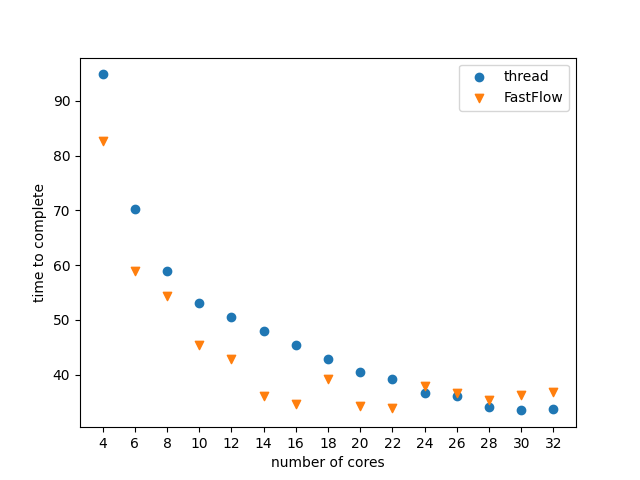
\includegraphics[width=0.7\textwidth]{./images/time_to_complete.png}
    \caption{Time for encoding of a 8GB file of random characters, in seconds. Averaged over 10 runs.}
    \label{fig:time_to_complete}
\end{figure}

In the figure \ref{fig:time_to_complete} the completion time of the two parallel implementation is compared. The FastFlow result is quite surprising because it achieves the minimum time with only 16 threads, and starts to worsen the performance increasing the parallel degree. A similar behaviour can be observed with the native thread, wehere is not worth to increase the number of threads over 28. The same results can be seen under a differen prospective in the efficiency plot, figure \ref{fig:efficiency}. I suspect that the great efficiency of FastFlow with 16 cores is correlated with the architecture of the machine used for the experiments.


\begin{figure}
    \centering
    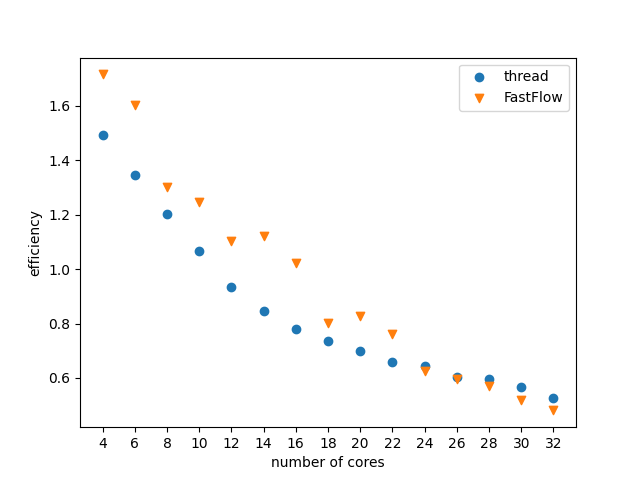
\includegraphics[width=0.7\textwidth]{./images/efficiency.png}
    \caption{Efficiency in the encoding of a 8GB file of random characters. Averaged over 10 runs.}
    \label{fig:efficiency}
\end{figure}

From the figure \ref{fig:efficiency} we can also observe that the efficiency is greater than one. This can happen when the speedup is greater than the parallel degree because the original problem became much easier when it is divided into subproblems. It might be that allocate and work a single 8 GB block is much slower than allocate 32 different 256 MB blocks, especially with the optimizations made by the jemalloc library and FastFlow. For example could happen that the sequential process allocates the memory on the RAM bank attached to the curren core and then is moved to another core or even anoter socket causing a lot of delay in accessing memory; in the parallel process is more likely that each tread allocate the memorory on the nearest RAM bank and then remains pinned to the same core.

These are only hypothesis difficult to verify, however the test reported in table \ref{tab:jemalloc} shows how important is the use of the jemalloc library for these implementations, expecially with FastFlow, that suffers by an order of magnitude the unoptimized standart library. This could partially explain the superlinear speedup observed before.

This result deservers further investigation, in table \ref{tab:ff_times16} the same test of table \ref{tab:ff_times} is repeated with 16 cores. Results show that the efficiency is surprisingly high since the speedup is almost linear. The $0.9 $ efficiency in \textit{compressing and writing} stage, shows that we are near the bandwidth of the disk and the $1.06$ efficiency in the \textit{encoding} stage is probably due to hypothesis above.

\begin{table}[!h]
    \begin{center}
    \begin{tabular}{c c c c}
        & \textbf{malloc} & \textbf{jemalloc} & speedup\\
        \hline
        \textbf{threads} & 196 s (169339515 $\mu s$)  & 33.3 s  (33328868 $\mu s$) & 5.08 x \\
        \hline
        \textbf{FastFlow} &  415 s  (414727131 $\mu s$) & 36.2 s (36295647 $\mu s$ ) & 11.42 x \\
        \hline
    \end{tabular}
\caption{Time to encode a 8GB file of random characters. Standart malloc library vs jemalloc. 32 physical core machine. Averaged over 10 runs. The term ``speedup'' here has a different meaning than the usual one: it is the ratio between the time with the standart library and the time with jemalloc.}    
\label{tab:jemalloc}
\end{center}
\end{table}


\begin{table}[h]
    \begin{center}
    \begin{tabular}{l c c c}
        \textbf{Stage} & \textbf{Time} & \textbf{Speedup} & \textbf{Efficiency}  \\
        \hline
        read and count & 1.6 s (1633635 $\mu s$)  & 15.87 x & 0.99  \\
        \hline
        huffman & 0.000095 s (95 $\mu s$) & \\
        \hline
        encoding & 12.5 s (12521952 $\mu s$)  & 16.96 x & 1.06 \\
        \hline
        balancing & 0.000027 s (27 $\mu s$ ) & \\
        \hline
        compressing and writing & 22 s (22056740 $\mu s$)  & 14.04 x & 0.90\\
        \hline
        \textbf{Total} & 38.7 s (38714097 $\mu s$)  & 14.64 x & 0.92 \\ 
\end{tabular} 
\caption{Parallel times with FastFlow implementation for 8GB file of random characters. 16 physical core machine. Averaged over 10 runs.}    
\label{tab:ff_times16}
\end{center}
\end{table}


\begin{figure}
    \centering
    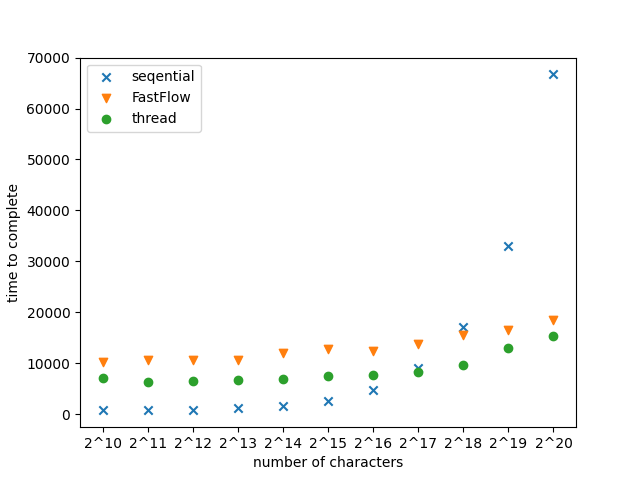
\includegraphics[width=0.7\textwidth]{./images/small._files.png}
    \caption{Time for encoding different sized files of random characters, in $ \mu s$, with 32 physical cores. Averaged over 10 runs.}
    \label{fig:small_files}
\end{figure}

It is useful to know when it is worth to use a parallel implementation instead of a sequential one. Give a precise answer to this question is difficult because the variables involved are many (file size, single core speed, parallel degree, etc.). However, in figure \ref{fig:small_files} we can see the time to encode different sized files fixing the number of workers to 32. We can see that with half a milion characters the parallel implementations are already faster than the sequential one. After the consideration made above about the efficiency, we can imagine that reducing a bit the number of workers reduces the overhead without increasing the completion time, so it would become useful to use parallel implementations even with smaller files.




\newpage \FloatBarrier
\bibliographystyle{plain}
\bibliography{bibliography}


\end{document}
